\documentclass{article}
% all of package must declartion in tex begin, this command means that using amsmath some feature
\usepackage{amsmath}
% this package support Chinese
\usepackage[UTF8]{ctex}
% this package support graph in latex
\usepackage{graphicx}
% this package support sub figure in  latex
\usepackage{subcaption}
% 设置目录中标题的间距
\usepackage{setspace}
% 设置表格需要跨多行的
\usepackage{multirow}
% 支持表格的上下表格线
\usepackage{booktabs}
% 旋转打印表格的包
\usepackage{rotating} 
\usepackage{tikz} % To generate the plot from csv
\usepackage{circuitikz} % draw circuit
 \usepackage{pgfplots}
\usepackage{siunitx} %显示SI国际物理单位的包
\usepackage{listings} %显示源代码
\usepackage{color}
\usepackage{hyperref} %用于超链接的包
\usepackage{enumitem}  % 用于有序列表前缀显示的包


\title{La\TeX \quad Notebook} % \quad是空格
\date{2020-01-05}
\author{george zzzh}

\begin{document}
	% 预先设置内容
	\pgfplotsset{compat=newest} % Allows to place the legend below plot
	\usepgfplotslibrary{units} % 允许输入单位
	\hypersetup{hidelinks} % 设置链接的颜色,隐藏链接上的红框
	\pagenumbering{gobble} % this gobble command is that disappear number in paper bottom
	\maketitle %this command is show title, date and author in first page
	\newpage 	% this command is make a new page
	\pagenumbering{Roman} % bring back the number on the bottom of paper
	\doublespacing 	% 设置目录间的间距
	\setcounter{tocdepth}{3} 	% 目录章节, 设置总体的目录深度
	\tableofcontents
	\newpage
	% 包含两个文件
	\section{安装教程}
详细参考这个网站, www.latex-tutorial.com
\subsection{TexWorks字体设置}
TexWorks中编辑-首选项-编辑器默认配置(字体),设置好之后,重启生效。
\section{一级标题}
section, table of content 是目录的意思。
\subsection{二级标题}
subsection.
\subsubsection{三级标题}
subsubsection. 
\paragraph{段落}
paragraph
\subparagraph{子段落}
Subparagraph, 
LaTex中层次分为5层,[section, subsection, subsubsection, paragraph, subparagraph],五个层次,可以在设置目录中显示要在目录中显示的层次,其中0代表什么都不显示,5代表显示到subparagraph
% 单独的设置目录的深度为1
\addtocontents{toc}{\setcounter{tocdepth}{1}}
\section{第二个标题,Another section}
\subsection{第二个子标题 Eat}
Eatting is necessary for human!
% 重新设置目录的深度为3
\addtocontents{toc}{\setcounter{tocdepth}{3}}
\section{数学公式, Math}
This is math envirment.
\begin{equation}
f(x)=x^2
\end{equation}
The following equation use amsmath package feature, the feature is that there isn't number beside equation.
\begin{equation*}
g(x)=\sum_{i=1}^{100}i
\end{equation*}
\section{数学公式}
接下来写几个数学公式,描述数学公式在LaTex中的使用
\subsection{行内公式写法,用\$作定界符号}
嵌入文本中的公式用\$包围,e.g. $1=\frac{1}{1}$ 嵌入完毕
\subsection{公式环境}
有equation和align两种环境, equation环境用于一个公式的排版,align可以写多行公式,会根据\&符号的位置对齐上下两个式子,$\backslash\backslash$用来换行。

\begin{equation}
1+2=3
\end{equation}

\begin{align}
1+0 &=1\\
1&=2-1
\end{align}
以下列举几个公式的例子\\
\subsubsection{积分}
\begin{align}
F(x)=\int_a^b\frac{1}{\sqrt{3}}x^3
\end{align}
\subsubsection{矩阵}
矩阵,用\$号界定的环境之下,用\{matrix\}环境写入
$
\begin{matrix}                                      
1 & 0\\
0 & 1
\end{matrix}
$

当矩阵要写入左右括号时,引入$\backslash left[$会放大括号
$\left[
\begin{matrix}
1 & 0\\
0 & 1
\end{matrix}
\right]
$
\subsubsection{$\backslash$left(的作用}
输入普通的大括号(普通字符)
\begin{equation}
(\frac{1}{\sqrt{x}}) 
1=2+-1
\end{equation}

$\backslash$left(
\begin{equation}
\left( \frac{1}{\sqrt{x}} \right)
\end{equation}
% 插图章节
\section{插图}
插一张巫师3的配图
% 为图片环境设置浮动值,此设置能使得图片在当前tex位置
% h是(here)-与tex文档相同位置, t(top of page), b(bottom of page), p (on an extra page), !(will force the specified location,强制执行制定的命令)
\begin{figure}[h!]
	\includegraphics[width=\linewidth]{avatar.png}
	\caption{picture about my avatar}
	%主要是为了标注一个图片,方便于引用
	\label{fig:qqavatar}
\end{figure}  

\subsection{引用图片示例 }
Figure \ref{fig:qqavatar} shows a picture on here!
\subsection{subfigure子图}
使用子图,需要用usepackage\{subcaption\}包, 此外就是subfigure环境了
\begin{figure}[h!]
	\centering
	\begin{subfigure}{0.4\linewidth}
		\includegraphics[width=\linewidth]{avatar.png}
		\caption{avatar}
	\end{subfigure}
	\begin{subfigure}{0.4\linewidth}
		\includegraphics[width=\linewidth]{avatar.png}
		\caption{also avatar}
	\end{subfigure}
	\begin{subfigure}{0.6\linewidth}
		\includegraphics[width=\linewidth]{avatar.png}
		\caption{avatar copy}
	\end{subfigure}
	\caption{two character of qq avatar}
	\label{fig:avatar}
\end{figure}


% 引用章节
\section{引用BibTeX}
随便的引用的BOOK \cite{DUMMY:1} ,嵌入在文本中;引用的ARTICLE \cite{ARTICLE:1},引用的INBOOK例子\cite{BOOK:2},引用因特网WEBSITE\cite{WEBSITE:2}的\cite{WEBSITE:1}
% 脚注章节
\section{脚注}
This is some example text\footnote{\label{myfootnote}脚注的具体内容,写在页面最下方}。textsuperscript是在文本右上有一个小角标,我在这里再次引用上面提到的脚注\textsuperscript{\ref{myfootnote}}。
% table章节
\section{table}
LaTeX中表格通过table环境和tabular环境的结合来创建。table环境负责定义表格的位置和对齐方式。表格真正的内容包括在tabular环境中。textbf\{\}是用来划定列数的。用在首行。
\begin{table}[h!]
	\begin{center}
		\caption{Your first table} %表格的说明文字
		\label{tab:table1}
		\begin{tabular}{l|c|r|l}
			\textbf{value 1} & \textbf{value 2} & \textbf{value 3} & \textbf{value 4}\\
			\hline
			1 & 1110.1 & a & 100 \\
			\hline
			2 & 10.1    & b  & 7
		\end{tabular}
	\end{center}
\end{table}
\subsection{跨多行的表格}
跨多行的表格,需要用usepackage\{multirow\},  multirow\{NUMBER OF ROW\} \{宽度( $\ast$为自动计算)\}\{内容\}
\begin{table}[h!]
	\begin{center}
		\caption{support table of multirow cell } %表格的说明文字
		\label{tab:table2}
		\begin{tabular}{l|c|r|l} %l表示left对齐, c表示center, r表示right
			\textbf{value 1} & \textbf{value 2} & \textbf{value 3} & \textbf{value 4}\\
			\hline
			\multirow{2}{*}{12} &1111.2 & d & 10\\
			                                     & 1110.1 & a & 100 \\
			\hline
			2 & 10.1    & b  & 7
		\end{tabular}
	\end{center}
\end{table}
\subsection{跨多列的表格}
多列控制命令, multicolumn\{Number of column\}\{Alignment,对齐方式\}\{content\}
\begin{table}[h!]
	\begin{center}
		\caption{Your first table} %表格的说明文字
		\label{tab:table3}
		\begin{tabular}{l|c|r|l}
			\textbf{value 1} & \textbf{value 2} & \textbf{value 3} & \textbf{value 4}\\
			\hline
		      \multicolumn{2}{c|}{120}  & a & 100 \\
			\hline
			2 & 10.1    & b  & 7
		\end{tabular}
	\end{center}
\end{table}
\subsection{多行多列结合的表格}
具体使用看以下code
\begin{table}[h!]
	\begin{center}
		\caption{Your first table} %表格的说明文字
		\label{tab:table4}
		\begin{tabular}{l|c|r|l}
			\toprule
			\textbf{value 1} & \textbf{value 2} & \textbf{value 3} & \textbf{value 4}\\
			\hline
			\multicolumn{2}{c|}{\multirow{2}{*}{1234}} & a & 100 \\
			\multicolumn{2}{c|}{} &c & 101\\
			\hline
			2 & 10.1   & b  & 7\\
			\bottomrule %该命令画出的线是粗的,而hline是细的,注意在最后画线的时候,上一行要进行换行\\
		\end{tabular}
	\end{center}
\end{table}

\subsection{旋转表格}  %不太懂为什么旋转表格总是新起一页打开
使用sidewaystable环境可以解决表格横向打印。
\begin{sidewaystable}[ph!]
	\begin{center}
		\caption{Landscape table.} %表格的说明文字
		\label{tab:table5}
		\begin{tabular}{l|c|r}
			\toprule
			\textbf{value 1} & \textbf{value 2} & \textbf{value 3}\\
			\midrule
			1 & 1110.1 & a  \\
			\hline
			2 & 10.1    & b  \\
			\bottomrule
		\end{tabular}
	\end{center}
\end{sidewaystable}
\subsection{超长表格}
有些表格是跨页的,使用usepackage\{longtable\}可以解决这个问题。具体参考网页\footnote{\label{multipage_table}https://www.latex-tutorial.com/tutorials/tables/}中的Multipage tables.
	\section{用.csv文件绘制table}
这节做的不理想,经常报错。略过。
\section{用.csv文 件简单绘图}
\begin{figure}[h!]
  \begin{center}
    \begin{tikzpicture}
      \begin{axis}[
          width=\linewidth, 
          grid=major, % 显示网格
          grid style={dashed,gray!30}, % Set the style
          xlabel=X Axis $U$, % Set the labels
          ylabel=Y Axis $I$,
          x unit=\si{\volt}, % 设置单位
          y unit=\si{\ampere},
          legend style={at={(0.5,-0.2)},anchor=north}, % 在图下显示图例
          x tick label style={rotate=90,anchor=east} % 显示横坐标
        ]
        \addplot 
        % the .csv file (on top), 注意.csv文件中前两行的名字与x,y的名字相一致
        table[x=column 1,y=column 2,col sep=comma] {second/table.csv}; 
        \legend{Plot}
      \end{axis}
    \end{tikzpicture}
    \caption{My first autogenerated plot.}
  \end{center}
\end{figure}
\section{tikz绘制矢量图}
mindmaps是思维导图的意思,flowchart流程图。
\begin{figure}[h!]
	\begin{center}
		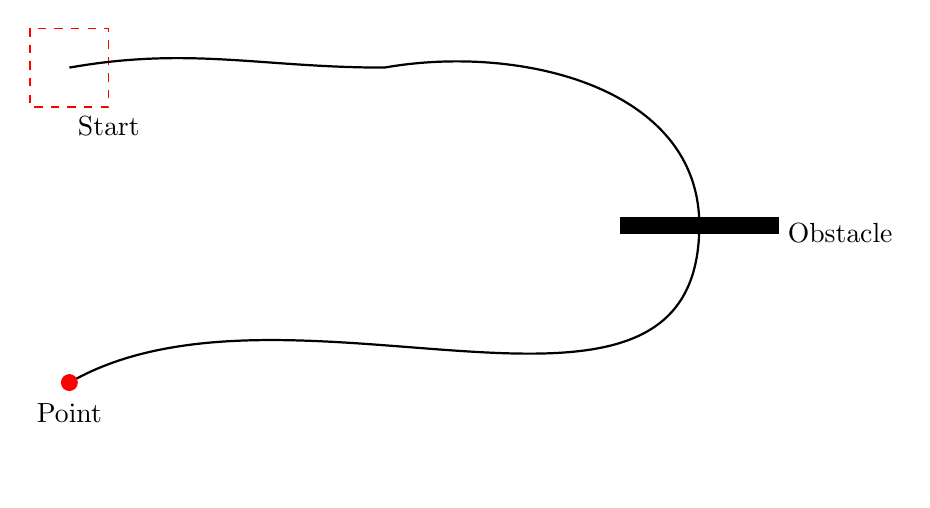
\begin{tikzpicture}
		     % 画矩形是确定对角线两点的坐标,start是字体
			\draw[red,dashed](-2.5,2.5) rectangle (-1.5,1.5)  node[black,below]{Start};
			\draw[thick](-2,2) 
			%设置入和出的角度,出是(-2,2)的出角度,入是进入(2,2)的角度,角度是按照极坐标系来算
			to [out=10,in=180] (2,2)
			to[out=10,in=90] (6,0)
			to[out=-90,in=30](-2,-2);
			\draw[fill](5,0.1) rectangle(7,-0.1) node[black,right]{Obstacle};
			\draw[red,fill] (-2,-2)  circle[radius=0.1] node[black,below=4]{Point};
		\end{tikzpicture}
	\end{center}
\end{figure}
\section{高亮源代码}
用listings包可以解决源代码高亮。
% \renewcommand\lstlistingname{Quelltext}
% 设置源代码区域显示格式
注意必须设置源代码中的注释和关键字的颜色,否则输出只有黑色和白色。
源代码包含在listings环境中。直接在LaTeX中写代码,遇到注释$\backslash\backslash$和$\ast$需要转义。
\lstset{
	language=Java,
	basicstyle=\small\sffamily,
	numbers=left,
	numberstyle=\tiny,
	frame=tb,
	tabsize=4,
	columns=fixed,
	showstringspaces=false, %在字符串的空格中显示一个下划线_
	showtabs=false, %在tab显示一个下划线_
	keepspaces=true, % keeps spaces in text, useful for keeping indentation of code (possibly needs columns=flexible), 暂且不知道什么作用
	commentstyle=\color{green},
	keywordstyle=\color{blue}
}
\begin{lstlisting}
public class Hello{
	public static void main(String[]args){
			System.out.println(''hello  world!'');
	}
}
\end{lstlisting}
再写一段代码, 也可以直接输入源代码的文件,而避免在LaTeX文档中输入代码。也不用注意代码中触及到LaTeX的关键字。
\lstinputlisting{second/hello.java}
\section{circuitikz绘制电路图}
\subsection{绘制基本电路图}
\begin{figure}[h!]
	\begin{center}
		\begin{circuitikz}
			\draw(0,0)
			to[V=$U_q$] (0,2)  % 电压源
			to[short] (2,2)          % 导线
			to[R=$R_1$] (2,0)  % 电阻
			to[short] (0,0) ;
			\draw (2,2)
			to[short] (4,2)
			to[L=$L_1$] (4,0)
			to[short] (2,0);
			\draw (4,2)
			to[short] (6,2)
			to[C=$C_1$] (6,0)
			to[short] (4,0);
		\end{circuitikz}
		\caption{My first circuit}
	\end{center}
\end{figure}

\subsection{circuit的高级使用}
\begin{figure}[h!]
	\begin{center}
		\begin{circuitikz}
			\draw (-1,0) to[short ,o-o] (1,0); % 两端用空心圆点连接
			\draw (0,0) to [short] node[ground] {GND} (0,-1);  %画出接地的标识
			\draw (-1,1) to[short ,*-] (1,1);   %两端用实心圆点和无圆点连接
		\end{circuitikz}
	\end{center}
\end{figure}

\subsection{画电路流向}
方向是通过circuitikz默认决定的,但是我们可以覆写。
\begin{figure}[h!]
	\begin{center}
		\begin{circuitikz}
			\draw (0,0) to[R,i^<=$i_1$] (2,0); % <是指明电流流向,_是让i1文字标识在下面,^是标注在上面
			\draw (0,-2) to [R,v>=$u_1$] (2,-2); %指明电压方向
			\draw (0,-4) to [R,l=$R_1$] (2,-4); %画一个电阻, l标识label标签
		\end{circuitikz}
	\end{center}
\end{figure}
\subsection{三极管}
\begin{figure}[h!]
	\begin{center}
		\begin{circuitikz}
		\draw (0,0) node[npn](npn1) {}
		(npn1.base) node[anchor=east] {B}
		(npn1.collector) node[anchor=south,xshift=0.5cm] {C}
		(npn1.emitter) node[anchor=north] {E};
		\draw (npn1.collector) to [R] ++(0,2); % (0,2)标识C端口的水平垂直位移
		\end{circuitikz}
	\end{center}
\end{figure}
\section{超链接hyperlink}
在MikTeX中编译包含hycolor.sty的时候,总是显示找不到hycolor.sty,在ctan中下载了hycolor.dtx之后, 执行以下命令
\begin{lstlisting}
$: tex hycolor.dtx
\end{lstlisting}
解压出hycolor.sty,放在.tex同一目录下,一起编译就可以。
\subsection{超链接}
超链接的蓝色的框,只在PDF显示中出现,在打印中不会出现。
这是个超链接,\href{http://www.baidu.com}{百度一下,你就知道}。
\subsection{URL}
嵌入一个简单的URL,\url{https://www.baidu.com}
\subsection{邮件地址}
邮件地址是: \href{george:usa@163.com}{usa@163.com}
\section{列表}
\subsection{无序列表}
\begin{itemize}
	\item One
	\item Two
	\item Three
\end{itemize}
\subsection{有序列表}
\begin{enumerate}
	\item One
	\item Two
	\item Three
\end{enumerate}
\subsection{嵌套列表}
\begin{enumerate}
	\item One
	\begin{enumerate}
		\item o
		\item n
		\item e
	\end{enumerate}
	\item two
	\item three
\end{enumerate}
\subsection{无序列表前的装饰}
可以修改无序列表前的装饰,而不是默认的黑点
\begin{itemize}
	\item[$-$] Dash
	\item[$\ast$] Asterisk
\end{itemize}
另外一种修改的方法, 统一指定前缀装饰
\begin{itemize}[label=$\ast$]
	\item one
	\item two
	\item three
\end{itemize}
\subsection{修改有序列表的前缀}
加载enumitem包,可以修改为字母,数字,罗马数字等。
\subsubsection{罗马数字}
\begin{enumerate}[label=(\roman*)]
	\item one
	\item two
	\item three
\end{enumerate}
\subsubsection{阿拉伯数字}
\begin{enumerate}[label=(\arabic*)]
	\item one
	\item two
	\item three
\end{enumerate}
\subsubsection{字母}
\begin{enumerate}[label=(\alph*)]
	\item one
	\item two
	\item three
\end{enumerate}
	% 插图目录
	\section{插图目录}
	在附录中显示一系列的插图
	% 文件的末尾,为图的目录和所有参考文献
	\newpage
	\begin{appendix}
		\listoffigures
	\end{appendix}
	% 所有引用的bib文件的信息
	\bibliography{bib/cite,bib/arti,bib/inbook,bib/website,bib/website2}
	\bibliographystyle{ieeetr}
\end{document}